V tejto kapitole opíšem všetkú potrebnú teóriu, poznatky, metódy, ktoré sú potrebné alebo mi pomohli pri vypracovávaní témy zadania.

\section{Inšpirácia}
Už dlhší čas som mal chuť vytvoriť nejakú počítačovú hru. Rád som v pozícii hráča a tak som si chcel aj vyskúšať pohľad na hry z tej druhej strany a vyskúšať si aspoň v malom merítku s akými problémami sa vývojari stretávajú. V poslednej dobe ma začala zaujímať téma umelej inteligencie a tak téma tejto práce bola príjemným skĺbením mojich dvoch záujmov.

\section{Plánovanie}
Plánovanie je problém alebo oblasť, ktorou sa zaoberá umelá inteligencia. Je to proces hľadania postupnosti akcií, ktoré sa majú vykonať aby sa dosiahlo vytýčeného cieľa. Je základným stavebným kameňom v problematike zadanej témy a teda upresním nejaké základné definicie z tejto oblasti.
\subsection{Fluent}
Fluent je vo všeobecnosti niečo, čo dokáže plynúť ako tekutina\cite{approach}. V našom ponímaní je to objekt, ktorý opisuje či niečo platí alebo nie a je schopný sa meniť časom. Je to niečo podobné ako predikáty z prvorádovej logiky.
\subsection{Stav}
Stav je definícia, opis sveta alebo objektu s ktorým pracujeme. Príbeh bude vlastne tvorený zmenou z jedného stavu herného sveta do druhého. Tieto zmeny sa uskutočňujú pomocou akcií.
\subsection{Akcia}
Akcia obsahuje predpoklady a dôsledky. Predpoklady sú nejaké podmienky alebo stav, ktorý musí byť splnený aby sa daná akcia mohla vykonať. Dôsledky na druhej strane sú efekty, ktoré ovplyvnia aktuálny stav sveta alebo iného objektu na ktorom sa akcia vykonáva. Pomocou akcií sa bude posúvať príbeh a vyvýjať postavy.
\subsection{Riešenie/Plán}
Nakoniec k riešeniu (plánu) sa dostávame zadefinovaním počiatočného a koncového stavu (cieľa) a nasledným prechádzaním akcií, ktoré možno vykonať až kým nedosiahneme cieľa.Teda riešenie plánovania (plán) je neprerušená postupnosť akcií z počiatočného stavu do cieľa.\\
Jedna z reprezentácii ako definovať vzťahy medzi týmito pojmami sú grafové štruktúry. V našom príklade to bude strom.
\begin{figure}[ht] 
\begin{center}
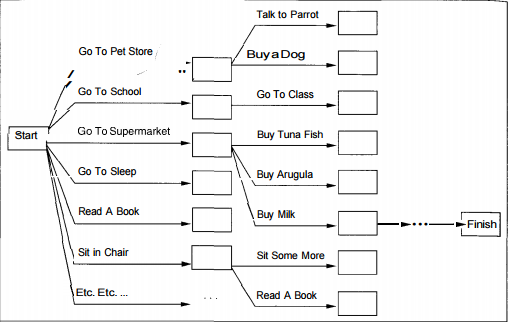
\includegraphics[scale=1.0]{img/plan.png}
\caption{Ukážka reprezentácie stavov a akcií \cite{approach}}
\label{fig:ch21}
\end{center}
\end{figure}
Na obrázku 2.1 môžeme vidieť stavy definované ako vrcholy grafu a akcie ako hrany medzi nimi. Máme počiatočný stav Start a koncový stav Finish. V tomto prípade je našim cieľom získanie mlieka. A teda v stave Start už máme definované fluenty a počiatočný stav sveta. Potom vhodným grafovým prehľadávacím algoritmom vieme hľadať postupnosť akcií a stavov pomocou, ktorých sa dostaneme z počiatočného stavu do koncového. Teda riešenie tohto plánovacieho problému je vlastne cesta v grafe začínajúca vo vrchole Start a končiaca vo vrchole Finish. Táto cesta nám teda hovorí, že na dosiahnutie nášho cieľa (získanie mlieka), musíme ísť do supermarketu a v ňom kúpiť mlieko. Riešení by mohlo byť aj viac ak by sme mali iný graf alebo doplnili do tohto nové akcie a stavy.

\section{Výpočtová naratológia}
Naratológiu ako pojem prvý krát zaviedol Tzvetan Todorov, bulharsko-francúzsky filozof, historik, sociológ a literárny kritik. Je to humanitná disciplína, ktorá sa zaoberá štúdiom narácie, teda príbehu alebo postupnosti udalostí \cite{narrat}. Ďalej skúma štruktúru, logiku, princípy a tiež aj reprezentáciu narácie. Zo začiatku dominovali štrukturálne prístupy štúdia z ktorých sa vyvynuli rôzne teórie, koncepty a analytické procedúry. Tieto koncepty a modely sú používané ako heuristické nástroje a naratologické teórie hrajú kľúčovú roľu v našej schopnosti vytvárať a spracovávať narácie vo všetkých možných formách. Čo nás privádza k umelej inteligencii a výpočtovej naratológii.\par
Výpočtová naratológia študuje tvorbu príbehov z pohľadu vypočítateľnosti a spracovávania informácií. Zameriava sa na algoritmické procesy, ktoré vytváraju a interpretujú príbehy a tiež na modelovanie štruktúry príbehu z hľadiska vypočítateľných reprezentácií. Sem patria aj spôsoby automatickej interpretácie a tvorby príbehov, daľej aj prístupy k rozprávaniu príbehov pomocou umelej inteligencie v hrách. Teda výskumníci sa snažili vytvoriť systémy umelej inteligencie, ktoré by rozprávali príbeh ako ľudia a tiež sa pokúšali vytvoriť inteligentné počítačové prostredie na interakciu s naráciami. V rámci vývoja týchto systémov, výskumníci využili princípy z naratológie na vytvorenie výpočtových princípov a vysvetlili prepojenia medzi nimi. Jeden z príncípov bolo využitie naratologického rozdelenia fabuly a sujetu. Kde fabula je zvyčajne charakterizovaná ako prirodzený sled udalostí celého príbehu v chronologickom poradí. Sujet na druhú stranu je umelecky realizovaná fabula, teda je to konštrukcia epickej alebo dramatickej fabuly. Výpočtová naratológia bola významne ovlplyvnená aj lingvistikou napríklad gramatikami pribehov. Je to rýchlo rozvíjajúce sa odvetvie, hľavne vďaka zvýšenému záujmu o interaktívne hry a príbehy, ktoré sa javia ako živé.
\section{Systémy generujúce príbehy}
Systémy generujúce príbehy vznikali ako odpoveďe na otázky výpočtovej naratológie. Hľadaním všeobecných vypočtových metód, ktoré by sa dali použiť na rôzne druhy narácie sa v 70-tych rokoch 20. storočia upriamila pozornosť na plánovanie. Odvtedy sa toto zameranie veľmi nezmenilo, ale plánovacie techniky sa vylepšili aby mohli poňať obsiahle problémy naratológie.\par
V problematike plánovania, na pochopenie príbehu je potrebné vyvodenie založené na Aristotelovom ponímaní mýtu, kde príčiny udalostí príbehu a cieľe zapojených postáv su známe. V podstate zrekonštruovať z viet v sujete plán, ktorý reprezentuje súslednosť udalostí, ktoré dokážu počiatočný stav transformovať na cieľový. Takéto systémy, ktoré sa snažia pochopiť príbeh sa nedostali veľmi daľeko z troch dôvodov. Po prvé, vyvodenie cieľov zainteresovaných postáv si vyžaduje obrovský priestor na prehľadávanie. Daľej, ľudia využívaju obrovské množstvo znalostí na pochopenie aj tých najjednoduchších príbehov. Príkladom nám môže byť veta od anglického spisovateľa Edwarda Morgana Fostera: "Kráľ zomrel a kráľovná zomrela od žiaľu.", z ktorej nám ľudom je jasné prečo bola kráľovná smutná, avšak definovať takúto dávku zdravého rozumu počítaču je náročné. Po tretie, niektoré aspekty jazyka, ktoré sú pre pochopenie príbehu dôležité, sa tažko formalizujú ako napríklad humor, irónia a iné nepatrné lexikálne prostriedky. Na druhú stranu algoritmy, ktoré využívajú na generovanie príbehu plánovanie pomocou fabuli sa osvedčili oveľa viac aj preto že si autor môže výrazne obmedziť systém. O takýchto algoritmoch si v tejto sekcii povieme viac.\par
\subsection{Novel Writer system}
Prvý storytellingový systém, ktorý bol zaznamenaný je Novel Writer system\cite{novel_writer} od Sheldona Kleina. Vytváral príbehy o vražde na víkendovej oslave. Údajne vedel vygenerovať 2100 slovné príbehy o vražde, s hlbokou myšlienkou za menej ako 19 sekúnd. Ako vstup sa zadal opis sveta v ktorom sa mal príbeh odohrať a aj charakteristika postáv, ktoré vystupovali v príbehu. Vrah a obeť závyseli od charakterových čŕt tiež špecifikovaných ako vstup. Všetky možné motívy na vraždu boli obmedzené iba na chamtivosť, zlosť, žiarlivosť a strach. Príbeh bol vygenerovaný pomocou dvoch algoritmov. Prvým bola množina pravidiel, ktorá obsahovala všetky možné zmeny stavu sveta z akutuálneho stavu do nasledujúceho. Druhým bola postupnosť scén ktorá korešpondovala s typom príbehu, ktorý mal byť prerozprávaný. Nevýhodou bolo, že množina pravidiel vysoko obmedzovala typ príbehu, ktorý sa vedel generovať. Rozdiely v príbehu spočívali len v tom, kto koho zabil s čím a prečo a v tom kto objavil mrtvolu. \par
\subsection{Talespin}
Neskôr bol vyvinutý systém TALESPIN\cite{talespin}, ktorý generoval príbehy o lesných tvoroch. Na tvorbu príbehu sa postave zadal cieľ alebo zámer a následne sa zkonštruoval plán ktorým bol dosiahnutý daný cieľ. TALESPIN ako prvý využil charakterové cieľe ako spúšťače akcií. Taktiež tu bola po prvý krát využitá možnosť viacerých takýchto postáv, kde každá mala svoj zoznam cieľov, ktoré chce dosiahnuť. Čo dalo možnosť vymodelovať zložitejšie vzťahy medzi postavami, napr. sútaživosť, dominancia alebo vernosť. Tieto vzťahy potom slúžili ako predpoklady pre niektoré akcie a ako dôsledky pre ostatné akcie. Toto predstavovalo jednoduchý model motivácie postáv. Nakoniec sa vygenerovali charakterové črty postáv pomocou rôznych hodôt láskavosti, samoľúbosti, úprimnosti a inteligencie.\par
\subsection{Author}
Ďalej si povieme o programe AUTHOR\cite{author}, ktorý mal simulovať myseľ autora ako vymýšľa príbeh. Premisa tohto programu bola, že prostredie príbehu je vytvorené zdôvodnením udalostí pre ktoré sa autor už rozhodol, že budú súčasťou príbehu. Autor sám môže mať, pri vytváraní príbehu, nejaké cieľe, ktoré priíbehom chce dosiahnuť. A aj ak nemá tak je všeobecne známe, že pri vytváraní príbehu existujú nejaké podvedomé obmedzenia a cieľe tvorivého procesu. Pod týmto sa má na mysli napríklad, či je príbeh konzistentný, či je vierohodný, či postavy v príbehu sú uveriteľné alebo aj či pozornosť čitateľa je udržiavaná počas celého príbehu. Toto sa môže preniesť na nejaké podcieľe situácií v príbehu do ktorých chce autor zaviesť niektoré postavy z príbehu alebo do rolí ktoré jednotlivé postavy majú zahrať v príbehu. Môžme teda povedať, že príbeh sa dá chápať ako nejaký výsledok zložitej spleti autorových zámerov. Tieto zámery potom prispievajú ku štrukturovaniu príbehu a nejako riadia proces budovania príbehu. Avšak vo výslednom diele už niesu vidno.\par
\subsection{Universe}
O 2 roky neskôr prišiel systém UNIVERSE\cite{universe}, ktorý generoval scenáre pre radu epízód do telenovely v ktorej hralo rolu veľa postáv a plynulo viaceo súčastne prebiehajúcich a prekrývajúcich sa dejov. UNIVERSE bol prvým storytelingovým systémom, ktorý venoval špecialnu pozornosť na proces tvorby postáv. Komplexné dátové štruktúry boli použité na reprezentáciu postáv. Spolu s nimi bol použitý aj jednoduchý algoritmus, ktorý mal tieto štruktúry naplnit. Vačšina však ostala na použivateľovi. Tento systém bol skôr prostriedkom na prieskum sériového generovania príbehu ako na generovanie príbehu so začiatkom a koncom. Pôvodne bol zamýšľaný ako pomôcka spisovateľom s nádejou na postupnú tranformáciu na samostaný systém generovania príbehu. UNIVERESE priblížil otázku týkajúcu sa vytvárania fiktívneho sveta. Či by sa najprv mal vybudovať svet a potom do sveta vložit príbeh alebo či by príbeh mal riadiť konštruovanie sveta, kde by sa postavy, lokality a rôzne objeky vytvárali podľa potreby. Tu nastáva rozdiel medzi UNIVERSE-om a AUTHOR-om. Tvorca systému UNIVERSE sa priklonil ku prvej moznosti a implementoval vytváranie postáv nezávisle od deja a na druhej strane bol tvorca AUTHOR-u ktorý sa priklánal k druhej možnosti.\par
\subsection{Minstrel}
Ďaľší v chronologickom poradí, ktorý si spomenieme je počítačový program MINSTREL\cite{minstrel}. Tento program vytváral príbehy o Kráľovi Artušovi a jeho rytieroch okrúhleho stola. MINSTREL používal stavebné jednotky pozostávajúce z cieľov a plánov ako dosiahnuť dané cieľe. Tieto fungovali na dvoch rôznych úrovniach: autorské cieľe a cieľe vystupujúcich postáv. Vytváranie príbehu fungovalo na základe procesu, ktorý mal dve štádiá, ktoré zahrnovali najprv plánovacie štádium a potom štádium riešenia problémov, ktoré navyše opätovne využívalo vedomosti z predošlých príbehov. Každý beh programu bol založený na nejakej vete, ktorá slúžila ako jadro okolo, ktorého sa píbeh staval.  MINSTREL vytváral príbehy dlhé pól strany až jedna strana.\par
\subsection{Mexica}
MEXICA\cite{mexica} je počítačový model, ktorý bol vytvorený na skúmanie kreatívneho procesu tvorby príbehov. Jeho úlohou bolo vytvárať krátke príbehy o pôvodných obyvateľoch Mexica. Autor tohto modelu sa riadil hypotézou tvorby príbehu na základe dvoch stavov. Prvý je stav, kedy spisovateľ je silno angažovaný do produkcie materiálu pre dané dielo. V tomto stave sa spisovateľ spolieha na predošlé skúsenosti iné mentálne schémy a zároveň sa vyhýba úmyselnému plánovaniu a rôznym dejovým štruktúram na vývoj diela. V druhom stave spisovateľ analyzuje a hodnotí to, čo doteraz napísal a uvážlivo to skúma a pozmieňa. A teda táto hypotéza hovorí, že cyklus medzi tymito dvoma stavmi tvorí dôležitú časť tvorby príbehu.\par
Podobne teda bol aj zkonštruovaný program tohto modelu. Pozostáva z dvoch hlavých súčastí. Prvá je založená na množine predchádzajúcich príbehov, ktoré sú definované používateľom pomocou textového dokumentu. Vytvorí sa skupina dátových štruktúr, ktoré reprezentujú abstraktné schémy príbehu. V druhej časti sa program odkazuje na štruktúry vytvorené v prvej časti a program prechádza dvoma stavmi z udanej hypotézi na vytvorenie príbehu. Tento model bol prevratný v tom, že využíval na pohánanie a hodnotenie príbehu aj emocionálne prepojenia a napätia medzi postavami.
\subsection{Brutus}
Ďaľším zaujímavým programom, ktorý si spomenieme je BRUTUS\cite{brutus}. Tento program vytváral krátke príbehy o zrade. Zaujímavý bol v tom, že na tvorbu príbehu využíval logický model zrady. Tento model bol dosť rozsiahly na to, aby sa z neho dali vyvodzovať informácie, ktoré umožnovali tvorbu kvetnatých príbehov. Bol navrhnutý tak, aby vedel brať do úvahy aj veľké množstvo vedomostí o literatúre a gramatike. Príbehy, ktoré tento program vytváral obsahovali vlastnosti, aké by sme mohli nájsť v príbehoch vytvorených ľudmi napr. rôzne literárne trópy a dialógy. Tvorcovia programu ale podotkli, že BRUTUS vôbec nie je tvorivý program je to skôr výsledok reverzného inžinierstva príbehu, na ktorom potom sledovali, či dokáže vybudovať daný príbeh. Dalo by sa povedať, že to bolo skĺbenie kreativity a logiky.
\subsection{Fabulist}
Najnovším spomedzi spomínaných algoritmov je architektúra FABULIST\cite{fabulist}, ktorá automatizuje generovanie príbehu a jeho prezentáciu. Využíva techniku takzvaného upresňujúceho vyhľadávania na riešenie problému ohľadom generovania príbehu a na nájdenie zvučnej a uveriteľnej postupnosti akcií postáv, ktorá teda počiatočný stav pretransformuje na konečný. Túto techniku využíva IPOCL (Intent-based Partial Order Causal Link) plánovač, ktorý priniesli v tejto architektúre, ktorý okrem vytvorenia bežne znejúceho deja aj pojednáva o zámeroch postáv v príbehu identifikovaním možných cieľov pre danú postavu, ktoré vysvetľujú spravanie postavy a následne vytvára plánovacie štruktúry, ktoré vysvetľujú prečo sa tieto postavy zameriavaju na ich cieľ.
\section{Goal Oriented Action Planning}
Goal Oriented Action Planning (GOAP) teda cieľovo orientované plánovanie akcii, je systém umelej inteligencie, ktorý ľahko zabezpečí možnosti a nástroje na rozumné rozhodovanie sa pre agentov bez toho, aby sme museli udržiavať veľký a zložitý stavový automat. Umožňuje agentom naplánovať postupnosť akcií, ktoré dosiahnu ich cieľ. Táto postupnosť nezávisí len od cieľa ale aj od aktuálneho stavu sveta a stavu agenta. To znamená, že ak by sme dali rovnaký cieľ dvom rôznym agentom alebo dvom agentom v rôznom stave sveta, môžeme dostať úplne odlišné postupnosti akcií, čo robí umelú inteligenciu viac dynamickú a realistickú.\par
Tento systém vyniká v situáciach, kedy by nám vznikali pri riešení problému veľké a komplikované stavové automaty, kde sa často stáva, že so dôjde do bodu, kedy už nechceme pridávať nové akcie lebo by to vyvolalo priveľa vedľajších efektov a medzier v umelej inteligencii.
\begin{figure}[H] 
\begin{center}
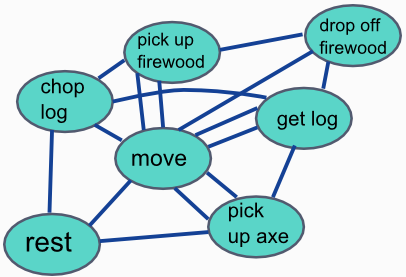
\includegraphics[scale=0.65]{img/fsm_states.png} \hspace{0.5cm}
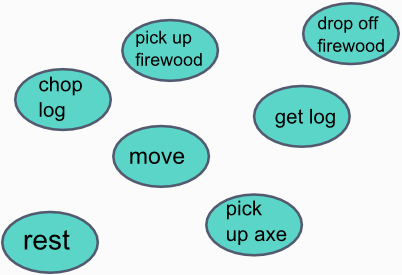
\includegraphics[scale=0.65]{img/goap_states.png}
\caption{Rozdiel medzi reprezentáciou pomocou stavového automatu a GOAP-u\cite{goap}}
\label{fig:ch22}
\end{center}
\end{figure}
GOAP teda umožnuje z ľavej časti obrázka 2.2 spraviť pravú, kde sú akcie samostatnou jednotkou a nezaoberajú sa vedľajšími efektami svojej činnosti. Tým, že sme jednotlivé akcie odpojili, tak sa môžme venovať každej zvlášť. Toto robí kód viac modulárnym a ľahšie sa testuje a udržiava. Ak by sme chceli pridať novú akciu, tak ju nám stačí pridať do našej reprezentácie a nijako to neovplyvní ostatné akcie, čo sa o reprezentácii stavovým automatom povedať nedá. Navyše rôzne akcie môžeme agentom pridávať a odoberať za behu. Aby sme pomohli GOAP-u zistiť aké akcie chceme vykonať, každá akcia dostane svoju cenu. Akciu s vysokou cenou nevyberieme namiesto akcie s cenou nižšou. Keď akcie usporiadame do postupnosti, sčítame hodnoty jednotlivých akcii, aby sme nakoniec mohli vybrať postupnosť s najnižšou cenou.\par
O toto sa stará GOAP plánovač, ktorý sa pozerá na predpoklady a dôsledky akcii a vytvára frontu akcii, ktoré spĺnajú náš cieľ. Cieľ je poskytnutý agentom spolu so stavom sveta v ktorom sa agent vyskytuje a zoznamom akcií, ktoré agent môže vykonať. S týmito informáciami potom plánovač môže skúšať vykonávať akcie, uvidí, ktoré sa dajú vykonať a ktoré nie a potom sa rozhodne, ktoré akcie je najlepšie vykonať. Plánovač neskončí hneď ako nájde prvú postupnosť, ktorá nás privedie do cieľa ale prejde aj ostatnými akciami, pretože sa môže stať že existuje iná postupnosť, ktorá má nižšiu cenu ako tá prvá. Teda prejde cez všetky možnosti aby našiel tú najlepšiu. Pri plánovaní sa buduje strom. Vždy keď plánovač použije nejakú akciu, tak ju vyhodí zo zoznamu akcií aby sa nestalo, že sa zacyklíme a chceme vykonávať tú istú akciu dookola. Následne sa zmení stav podľa dôsledku akcie. Keby sme mali za úlohu napr. získať drevo na oheň, tak by plánovací strom mohol vyzerať, tak ako popisuje obrázok 2.3.
\begin{figure}[H] 
\begin{center}
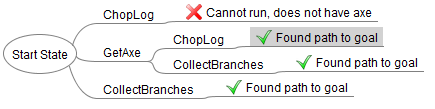
\includegraphics[scale=1.0]{img/plan_tree.png}
\caption{Plánovací strom GOAP plánovača \cite{goap}}
\label{fig:ch23}
\end{center}
\end{figure}
\section{Predošlé bakalárske práce}
Pri uvedení do problematiky a tvorbe bakalárskej práce mi boli nápomocné dve predošlé bakalárske práce. A to Tvorba interaktívnych príbehov ako plánovanie od Martina Zvaru a Tvorba zápletiek v dobrodružných hrách od Dominika Dobiáša.\par
Prvá spomenutá bakalárska práca je podobná mojej v tom, že tiež využíva plánovanie na generovanie príbehov. Táto práca používa ako základ zformalizovaný Proppov model ktorý je zapísaný ako plánovací problém a naprogramovaný ako logický program pomocou ASP. A na samotné generovanie príbehov bol použitý solver Clingo, ktorý bol spúštaný pomocou Javy. Jeden z rozdielov v našej práci je skutočnosť, že tu sa bude využívať len programovací jazyk Java a nie logické programovanie. Ďalší z rozdielov je, že na riešenie plánovania sa použije vlastný solver. Taktiež v spomenutej práci sa nehľadí na zaujímavosť generovaného príbehu. Touto problematikou sa naša práca zaujímať bude. A nakoniec tvorba príbehov v tejto práci bude zasadená do jednoduchej dobrodružnej textovej hry, kdežto v práci od pána Zvaru išlo čisto o program, ktorý generuje príbehy.\par
Druhá bakalárska práca, ktorú spomíname je našej viac podobná ako prvá spomenutá. Práca od pána Dobiáša taktiež rieši problematiku zaujímavosti príbehu a podobne ako naša práca tiež implementovala vlastný solver na generovanie príbehov. K rozdieľom patrí nepoužité GOAP plánovanie v práci pána Dobiáša a tiež vygenerovaný príbeh nebol vyjadrený vo forme hry.